\documentclass[a4paper]{article}

 \usepackage{fontenc}

\usepackage[english]{babel}
\usepackage[utf8]{inputenc}
\usepackage{amsmath, amsthm}
\usepackage{graphicx}
\usepackage[colorinlistoftodos]{todonotes}
\usetikzlibrary{trees}
\usepackage{geometry}
\usepackage{amssymb}
\usepackage{enumitem}
\usepackage{fancyhdr}
\usepackage{tikz}
\usetikzlibrary{trees}
\pagestyle{fancy}

\usepackage{comment}
\usepackage{float}
\usepackage{mathrsfs}
\usepackage{physics}
\usepackage{bbm}
\usepackage[hidelinks]{hyperref}
\usepackage{parskip}
\usepackage{lipsum}
\usepackage{pgfplots}
\usepackage{caption}
\usepackage{subcaption}

\theoremstyle{definition}
\newtheorem{definition}{Definition}
\newtheorem{example}{Example}
\newtheorem{remark}{Remark}

\theoremstyle{plain}
\newtheorem{lemma}{Lemma}
\newtheorem{proposition}{Proposition}
\newtheorem{theorem}{Theorem}
\newtheorem{corollary}{Corollary}

\renewcommand{\headrulewidth}{0pt}
\renewcommand{\footrulewidth}{0pt}

\newcommand{\approptoinn}[2]{\mathrel{\vcenter{
  \offinterlineskip\halign{\hfil$##$\cr
    #1\propto\cr\noalign{\kern2pt}#1\sim\cr\noalign{\kern-2pt}}}}}

\newcommand{\appropto}{\mathpalette\approptoinn\relax}

\begin{document}


{\center\Large\scshape Learning Feature Representations\par}
{\center\large\scshape Module 1 Homework\par}
\vspace{2mm}
{\center\scshape Oscar Carlsson\\Jimmy Aronsson\par}
\vspace{1mm}
{\center\small\scshape \today\par}
\vspace{7mm}
%\maketitle

In this document, we summarize our work on the first Homework.

\section*{\center Exercise 1}

In this first exercise, we attempt to model the (unknown) distribution of MNIST images, $x \sim p_d$, and hopefully generate synthetic images that look realistic. More precisely, we remove the empirical mean $\mu$ from each training image and see whether the remaining noise $x - \mu$ can be modeled with a multivariate Gaussian distribution $\mathcal{N}(\mathbf{0},\Sigma_\theta)$ with learned precision matrix $\Lambda_\theta = \Sigma_\theta^{-1}$. Synthetic images could then be created by either sampling noise from the model distribution and adding back the empirical mean, 
$$x' = \mu + \epsilon, \qquad \epsilon \sim \mathcal{N}(\mathbf{0},\Sigma_\theta),$$
or by using the precision matrix directly:
$$x' = \mu + A_\theta \epsilon, \qquad A_\theta = \Lambda_\theta^{-1/2}, \epsilon \sim \mathcal{N}(0,1/100).$$

Two different methods have been used to estimate the precision matrix:
\begin{itemize}
\item Noise-contrastive estimation (NCE), and
\item Score matching (SM).
\end{itemize}
Seeing as the underlying ideas and general analysis of these methods have already been discussed by Christopher Zach in his \texttt{presentation\_part1}, we shall gloss over the introductions and focus on those additional, important details which are not featured in the presentation.


\begin{figure}[H]
	\centering
	\begin{subfigure}[b]{0.49\textwidth}
		% This file was created by tikzplotlib v0.9.6.
\begin{tikzpicture}

\begin{axis}[
colorbar,
colorbar style={ytick={-2000,0,2000,4000,6000,8000,10000},yticklabels={−2000,0,2000,4000,6000,8000,10000},ylabel={}},
colormap/viridis,
point meta max=10241.4711396514,
point meta min=-2227.58785185868,
tick align=outside,
tick pos=left,
title={Empirical precision matrix for MNIST},
x grid style={white!69.0196078431373!black},
xmin=-0.5, xmax=783.5,
xtick style={color=black},
y dir=reverse,
y grid style={white!69.0196078431373!black},
ymin=-0.5, ymax=783.5,
ytick style={color=black}
]
\addplot graphics [includegraphics cmd=\pgfimage,xmin=-0.5, xmax=783.5, ymin=783.5, ymax=-0.5] {empirical_precision_matrix_minus_trained_for_mnist-000.png};
\end{axis}

\end{tikzpicture}

		\caption{}
	\end{subfigure}
	\hfill
	\begin{subfigure}[b]{0.49\textwidth}
		% This file was created by tikzplotlib v0.9.6.
\begin{tikzpicture}

\begin{axis}[
colorbar,
colorbar style={ytick={-2000,0,2000,4000,6000,8000,10000},yticklabels={-2000,0,2000,4000,6000,8000,10000},ylabel={}},
colormap/viridis,
point meta max=10216.2814405137,
point meta min=-2011.17676962237,
tick align=outside,
tick pos=left,
title={Zoomed-in, lower-right corner},
x grid style={white!69.0196078431373!black},
xmin=-0.5, xmax=69.5,
xtick style={color=black},
y dir=reverse,
y grid style={white!69.0196078431373!black},
ymin=-0.5, ymax=69.5,
ytick style={color=black},
scale=0.9
]
\addplot graphics [includegraphics cmd=\pgfimage,xmin=-0.5, xmax=69.5, ymin=69.5, ymax=-0.5] {Exercise1/Figures/last_70_elements_of_empirical_precision_matrix-000.png};
\end{axis}

\end{tikzpicture}

		\caption{}
	\end{subfigure}
	\caption{Empirical precision matrix for MNIST}
\end{figure}


\subsection*{NCE}

As explained in the presentation by Zach, noise-contrastive estimation (NCE) casts the estimation of distribution parameters as a supervised learning problem. This effectively means teaching the model distribution $p_\theta$ to distinguish between real data $x \sim p_d$ and noise data $x' \sim p_n$, where the noise distribution should be similar enough to the data distribution for this classification problem to be challenging; we want the model distribution $p_\theta$ to learn  the most essential properties of $p_d$.

After choosing a suitable noise distribution $p_n$, we construct a data set by flipping a weighted coin $z \sim \text{Bern}(1-\eta)$ multiple times and letting each result $z_i \in \{0,1\}$ decide whether to sample $x_i$ from the data distribution ($z_i = 1$) or from the noise distribution ($z_i = 0$). Denote the resulting training examples by $x_1,\ldots,x_N$ and noise samples by $x_1',\ldots,x_M'$, so that $M+N$ is the total number of coin flips. In NCE, we wish to use these samples to minimize the loss function

\begin{equation}\label{J_function}
J(\theta) \propto \mathbb{E}_{x \sim p_d} \left[ \log \frac{p_\theta(x)}{p_\theta(x) + \nu p_n(x)}\right] + \nu \mathbb{E}_{x \sim p_n} \left[ \log \frac{ \nu p_n(x)}{p_\theta(x) + \nu p_n(x)}\right],
\end{equation}


where $\eta = \frac{1}{1+\nu}$. We approximate the right-hand side of equation \eqref{J_function} using the empirical estimate
$$\frac{1}{N} \sum_{i=1}^N \log \frac{p_\theta(x_i)}{p_\theta(x_i) + \nu p_n(x_i)} + \frac{\nu}{M} \sum_{j=1}^M \log\frac{\nu p_n(x_j')}{p_\theta(x_j') + \nu p_n(x_j')},$$
which we simplify by rewriting both terms in the following way:
\begin{alignat*}{1}
\log \frac{p_\theta(x)}{p_\theta(x) + \nu p_n(x)} &= -\log\left( 1 + \nu \frac{p_n(x)}{p_\theta(x)}\right),\\
\log \frac{\nu p_n(x)}{p_\theta(x) + \nu p_n(x)} &= - \log \left( 1 + \frac{1}{\nu} \frac{p_\theta(x)}{p_n(x)} \right).
\end{alignat*}
If we now insert the relative probability
$$w(x) = \frac{p_n(x)}{p_\theta(x)}  = \sqrt{\frac{|\Lambda_n|}{|\Lambda_\theta|}} \exp\left( -\frac{1}{2} x^T \left( \Lambda_n - \Lambda_\theta\right) x\right),$$
then we obtain the relatively simple expression
\begin{equation}\label{J_function2}
J(\theta) \appropto -\frac{1}{N} \sum_{i=1}^N \log\left( \nu w(x_i) + 1\right) -\frac{\nu}{M} \sum_{j=1}^M \log\left(\frac {1}{\nu w(x_j')} + 1\right).
\end{equation}
We found that $w(x)$ is typically very small in practice, hence the sum $(\nu w)^{-1} + 1$ is dominated by its first term. Its logarithm can thus be approximated by the numerically more stable expression
\begin{alignat*}{1}
\log(\frac{1}{\nu w(x)} + 1) \approx -\log \nu w(x) = \frac{1}{2}x^T (\Lambda_n - \Lambda_\theta) x - \frac{1}{2} \log \left(\nu^2  \frac{|\Lambda_n|}{|\Lambda_\theta|}\right).
\end{alignat*}
It would also be possible to remove the first sum in equation \eqref{J_function2}, since $\log(\nu w(x) + 1) \approx \log 1$. We decided to keep it, however, because it didn't cause computational problems and we didn't want our estimate to be independent of the real training data. Thus, our final estimate is
$$\boxed{J(\theta) \appropto -\frac{\nu}{2}\log \left(\nu^2 \frac{|\Lambda_n|}{|\Lambda_\theta|}\right) -\frac{1}{N} \sum_{i=1}^N \log\left( \nu w(x_i) + 1\right) + \frac{\nu}{2M} \sum_{j=1}^M {x_j'}^T (\Lambda_n - \Lambda_\theta) x_j'}$$
We also obtained an expression for the gradient $\nabla J(\theta)$ in terms of the precision matrix $\Lambda_\theta$, though we found this expression rather bulky and difficult to handle. Instead, we used \texttt{tf.GradientTape} to compute the gradient and update $\Lambda_\theta$.  Two approaches were considered for keeping $\Lambda_\theta$ positive definite and retaining its sparse 4-/8-connected neighbourhood-structure after each epoch:
\begin{enumerate}
\item Writing the precision matrix as $\Lambda_\theta = (A_\theta ^T A_\theta) \cdot M$ for a learned matrix $A_\theta$ and a pre\-defined masking matrix $M \in \{0,1\}^{28\times 28}$ that is applied element-wise, enforcing the neighbourhood structure by killing undesired matrix elements.

The matrix product $A_\theta^T A_\theta$ is guaranteed to be symmetric positive definite whenever $A_\theta$ is invertible, which any square matrix almost surely is. Combined with the fact that element-wise products of positive definite matrices is again positive definite, we hoped this would prove that $\Lambda_\theta$ is symmetric positive definite. Unfortunately, we eventually realized that our masking matrix is not positive definite, so we cannot guarantee that $\Lambda_\theta$ is, either. Learning $A_\theta$ also turned out to be slower than the approach below.

\item Forcing a symmetric gradient by throwing away its lower triangular part and replacing it with the transpose of its upper triangular part. We then applied the previously mentioned masking matrix $M$ to force the neighbourhood structure on the gradient. This ensures that $\Lambda_\theta$ is symmetric and retains its neighbourhood structure for all epochs. On the other hand, we still cannot guarantee that $\Lambda_\theta$ remains positive definite.
\end{enumerate}
We ended up choosing the latter approach.\footnote{We later realized $\Lambda_\theta$ can also be modeled through its eigendecomposition, which would make it easy to ensure positive (semi)definiteness by flipping the signs of negative eigenvalues. Due to time constraints and different priorities, however, we never tried implementing this approach.}

$$\textit{*Insert figures of samples, loss, etc*}$$

\subsection*{Score Matching}

When given the choice between cNCE and score matching, we figured the latter would be more interesting, it being a fundamentally different approach than NCE. Fortunately, score matching also turned out to be easy to implement because the relevant analysis had already been excellently performed in the presentation. It allowed us to more or less directly implement the loss function
\begin{alignat*}{1}
J(\mu,\Lambda_\theta) &= \int \frac{1}{2} \|\nabla_x \log p_\theta(x)\|^2 + \Delta \log p_\theta(x) \approx \frac{1}{2N} \sum_{i=1}^N \| \Lambda_\theta (x_i - \mu)\|^2 - \tr(\Lambda_\theta),
\end{alignat*}
and start training. Gradients were again computed with \texttt{tf.GradientTape}, and the symmetry and neighbourhood structure was enforced in the same way as for NCE.

To get a better idea of how well our learned distribution $p_\theta$ approximates the data distribution $p_d$, we have created synthetic images in two different ways: (1) Sampling straight from a multivariate Gaussian $\mathcal{N}(\bar\mu,\Sigma_\theta)$ using the empirical mean $\bar\mu$ and the learned covariance matrix $\Sigma_\theta = \Lambda_\theta^{-1}$. (2) Following the instructions in the assignment by setting
$$x \leftarrow \bar\mu + \Sigma_\theta^{1/2}\varepsilon,$$
where $\varepsilon \sim \mathcal{N}(\mathbf{0},\mathbf{I})$. Combined with the choice of 4-/8-connected structure, this makes 4 different kinds of samples, which are shown in Figures \ref{samples_SM_fig1}-\ref{samples_SM_fig4}. An immediate observation is that 8-connected structure seems to produce better samples, which is reasonable considering it is more general than 4-connected structure and can better approximate the data distribution. That being said, while many samples contain digit-like shapes, they do not resemble  MNIST images.

Figures \ref{precision_matrix_SM_fig1}-\ref{precision_matrix_SM_fig2} show the learned precision matrix in the cases of 4-/8-connected structure, and finally, Figure \ref{loss_SM_fig} illustrates the loss in both cases.


%-----------------------------------------------------------------------------------------------------------------------------------------------------------------------------------------
% Removed samples with mu = 0 to lower the total number of figures.
\begin{comment}
\begin{figure}[H]
	\centering
	\begin{subfigure}[b]{0.3\textwidth}
		% This file was created by tikzplotlib v0.9.6.
\begin{tikzpicture}

\begin{axis}[
tick align=outside,
tick pos=left,
title={Sample form multivariate normal
 with \(\displaystyle \mu\)=0},
x grid style={white!69.0196078431373!black},
xmin=-0.5, xmax=27.5,
xtick style={color=black},
y dir=reverse,
y grid style={white!69.0196078431373!black},
ymin=-0.5, ymax=27.5,
ytick style={color=black}
]
\addplot graphics [includegraphics cmd=\pgfimage,xmin=-0.5, xmax=27.5, ymin=27.5, ymax=-0.5] {sample_0_using_multivariate_normal_with_mu_0_for_nce_False_with_orthogonal_mask-000.png};
\end{axis}

\end{tikzpicture}

	\end{subfigure}
	\hfill
	\begin{subfigure}[b]{0.3\textwidth}
		% This file was created by tikzplotlib v0.9.6.
\begin{tikzpicture}

\begin{axis}[
%colorbar,
%colorbar style={ylabel={}},
%colormap/viridis,
point meta max=0.5418341755867,
point meta min=-0.590289771556854,
tick align=outside,
tick pos=left,
title={},
x grid style={white!69.0196078431373!black},
xmin=-0.5, xmax=27.5,
xtick style={color=black},
y dir=reverse,
y grid style={white!69.0196078431373!black},
ymin=-0.5, ymax=27.5,
ytick style={color=black},
scale=0.5
]
\addplot graphics [includegraphics cmd=\pgfimage,xmin=-0.5, xmax=27.5, ymin=27.5, ymax=-0.5] {Exercise1/Figures/sample_1_using_multivariate_normal_with_mu_0_for_nce_False_with_orthogonal_mask-000.png};
\end{axis}

\end{tikzpicture}

	\end{subfigure}
	\hfill
		\begin{subfigure}[b]{0.3\textwidth}
		% This file was created by tikzplotlib v0.9.6.
\begin{tikzpicture}

\begin{axis}[
tick align=outside,
tick pos=left,
title={Sample form multivariate normal
 with \(\displaystyle \mu\)=0},
x grid style={white!69.0196078431373!black},
xmin=-0.5, xmax=27.5,
xtick style={color=black},
y dir=reverse,
y grid style={white!69.0196078431373!black},
ymin=-0.5, ymax=27.5,
ytick style={color=black}
]
\addplot graphics [includegraphics cmd=\pgfimage,xmin=-0.5, xmax=27.5, ymin=27.5, ymax=-0.5] {sample_2_using_multivariate_normal_with_mu_0_for_nce_False_with_orthogonal_mask-000.png};
\end{axis}

\end{tikzpicture}

	\end{subfigure}
	\caption{Samples drawn from $\mathcal{N}(\mathbf{0},\Sigma_\theta)$ with 4-connected precision matrix (SM).}
\end{figure}

\begin{figure}[H]
	\centering
	\begin{subfigure}[b]{0.3\textwidth}
		% This file was created by tikzplotlib v0.9.6.
\begin{tikzpicture}

\begin{axis}[
colorbar,
colorbar style={ylabel={}},
colormap/viridis,
point meta max=2.10015487670898,
point meta min=-1.66373884677887,
tick align=outside,
tick pos=left,
title={Sample form multivariate normal
 with \(\displaystyle \mu\)=0},
x grid style={white!69.0196078431373!black},
xmin=-0.5, xmax=27.5,
xtick style={color=black},
y dir=reverse,
y grid style={white!69.0196078431373!black},
ymin=-0.5, ymax=27.5,
ytick style={color=black}
]
\addplot graphics [includegraphics cmd=\pgfimage,xmin=-0.5, xmax=27.5, ymin=27.5, ymax=-0.5] {sample_0_using_multivariate_normal_with_mu_0_for_nce_False_with_eight_neighbours_mask-000.png};
\end{axis}

\end{tikzpicture}

	\end{subfigure}
	\hfill
	\begin{subfigure}[b]{0.3\textwidth}
		% This file was created by tikzplotlib v0.9.6.
\begin{tikzpicture}

\begin{axis}[
colorbar,
colorbar style={ylabel={}},
colormap/viridis,
point meta max=2.80104613304138,
point meta min=-2.01866793632507,
tick align=outside,
tick pos=left,
title={Sample form multivariate normal
 with \(\displaystyle \mu\)=0},
x grid style={white!69.0196078431373!black},
xmin=-0.5, xmax=27.5,
xtick style={color=black},
y dir=reverse,
y grid style={white!69.0196078431373!black},
ymin=-0.5, ymax=27.5,
ytick style={color=black}
]
\addplot graphics [includegraphics cmd=\pgfimage,xmin=-0.5, xmax=27.5, ymin=27.5, ymax=-0.5] {sample_1_using_multivariate_normal_with_mu_0_for_nce_False_with_eight_neighbours_mask-000.png};
\end{axis}

\end{tikzpicture}

	\end{subfigure}
	\hfill
		\begin{subfigure}[b]{0.3\textwidth}
		% This file was created by tikzplotlib v0.9.6.
\begin{tikzpicture}

\begin{axis}[
tick align=outside,
tick pos=left,
title={Sample form multivariate normal
 with \(\displaystyle \mu\)=0},
x grid style={white!69.0196078431373!black},
xmin=-0.5, xmax=27.5,
xtick style={color=black},
y dir=reverse,
y grid style={white!69.0196078431373!black},
ymin=-0.5, ymax=27.5,
ytick style={color=black}
]
\addplot graphics [includegraphics cmd=\pgfimage,xmin=-0.5, xmax=27.5, ymin=27.5, ymax=-0.5] {sample_2_using_multivariate_normal_with_mu_0_for_nce_False_with_eight_neighbours_mask-000.png};
\end{axis}

\end{tikzpicture}

	\end{subfigure}
	\caption{Samples drawn from $\mathcal{N}(\mathbf{0},\Sigma_\theta)$ with 8-connected precision matrix (SM).}
\end{figure}
\end{comment}
%-----------------------------------------------------------------------------------------------------------------------------------------------------------------------------------------

\begin{figure}[H]
	\centering
	\begin{subfigure}[b]{0.3\textwidth}
		% This file was created by tikzplotlib v0.9.6.
\begin{tikzpicture}

\begin{axis}[
%colorbar,
%colorbar style={ylabel={}},
%colormap/viridis,
point meta max=1.54649686813354,
point meta min=-0.40969842672348,
tick align=outside,
tick pos=left,
title={},
x grid style={white!69.0196078431373!black},
xmin=-0.5, xmax=27.5,
xtick style={color=black},
y dir=reverse,
y grid style={white!69.0196078431373!black},
ymin=-0.5, ymax=27.5,
ytick style={color=black},
scale=0.5
]
\addplot graphics [includegraphics cmd=\pgfimage,xmin=-0.5, xmax=27.5, ymin=27.5, ymax=-0.5] {Exercise1/Figures/sample_0_using_multivariate_normal_with_mu_pixel_val_for_nce_False_with_orthogonalmask-000.png};
\end{axis}

\end{tikzpicture}

	\end{subfigure}
	\hfill
	\begin{subfigure}[b]{0.3\textwidth}
		% This file was created by tikzplotlib v0.9.6.
\begin{tikzpicture}

\begin{axis}[
colorbar,
colorbar style={ylabel={}},
colormap/viridis,
point meta max=1.04302334785461,
point meta min=-0.61077219247818,
tick align=outside,
tick pos=left,
title={Sample form multivariate normal
 with \(\displaystyle \mu\)=mean(pixel\_val)},
x grid style={white!69.0196078431373!black},
xmin=-0.5, xmax=27.5,
xtick style={color=black},
y dir=reverse,
y grid style={white!69.0196078431373!black},
ymin=-0.5, ymax=27.5,
ytick style={color=black}
]
\addplot graphics [includegraphics cmd=\pgfimage,xmin=-0.5, xmax=27.5, ymin=27.5, ymax=-0.5] {sample_1_using_multivariate_normal_with_mu_pixel_val_for_nce_False_with_orthogonalmask-000.png};
\end{axis}

\end{tikzpicture}

	\end{subfigure}
	\hfill
		\begin{subfigure}[b]{0.3\textwidth}
		% This file was created by tikzplotlib v0.9.6.
\begin{tikzpicture}

\begin{axis}[
colorbar,
colorbar style={ylabel={}},
colormap/viridis,
point meta max=1.35305666923523,
point meta min=-0.521333932876587,
tick align=outside,
tick pos=left,
title={Sample form multivariate normal
 with \(\displaystyle \mu\)=mean(pixel\_val)},
x grid style={white!69.0196078431373!black},
xmin=-0.5, xmax=27.5,
xtick style={color=black},
y dir=reverse,
y grid style={white!69.0196078431373!black},
ymin=-0.5, ymax=27.5,
ytick style={color=black}
]
\addplot graphics [includegraphics cmd=\pgfimage,xmin=-0.5, xmax=27.5, ymin=27.5, ymax=-0.5] {sample_2_using_multivariate_normal_with_mu_pixel_val_for_nce_False_with_orthogonalmask-000.png};
\end{axis}

\end{tikzpicture}

	\end{subfigure}
	\caption{Samples drawn from $\mathcal{N}(\bar\mu,\Sigma_\theta)$ with 4-connected precision matrix (SM).}
	\label{samples_SM_fig1}
\end{figure}


\begin{figure}[H]
	\centering
	\begin{subfigure}[b]{0.3\textwidth}
		% This file was created by tikzplotlib v0.9.6.
\begin{tikzpicture}

\begin{axis}[
colorbar,
colorbar style={ylabel={}},
colormap/viridis,
point meta max=2.7683789730072,
point meta min=-1.21244716644287,
tick align=outside,
tick pos=left,
title={Sample form multivariate normal
 with \(\displaystyle \mu\)=mean(pixel\_val)},
x grid style={white!69.0196078431373!black},
xmin=-0.5, xmax=27.5,
xtick style={color=black},
y dir=reverse,
y grid style={white!69.0196078431373!black},
ymin=-0.5, ymax=27.5,
ytick style={color=black}
]
\addplot graphics [includegraphics cmd=\pgfimage,xmin=-0.5, xmax=27.5, ymin=27.5, ymax=-0.5] {sample_0_using_multivariate_normal_with_mu_pixel_val_for_nce_False_with_eight_neighboursmask-000.png};
\end{axis}

\end{tikzpicture}

	\end{subfigure}
	\hfill
	\begin{subfigure}[b]{0.3\textwidth}
		% This file was created by tikzplotlib v0.9.6.
\begin{tikzpicture}

\begin{axis}[
%colorbar,
%colorbar style={ylabel={}},
%colormap/viridis,
point meta max=1.88314282894135,
point meta min=-0.814143598079681,
tick align=outside,
tick pos=left,
title={},
x grid style={white!69.0196078431373!black},
xmin=-0.5, xmax=27.5,
xtick style={color=black},
y dir=reverse,
y grid style={white!69.0196078431373!black},
ymin=-0.5, ymax=27.5,
ytick style={color=black},
scale=0.5
]
\addplot graphics [includegraphics cmd=\pgfimage,xmin=-0.5, xmax=27.5, ymin=27.5, ymax=-0.5] {Exercise1/Figures/sample_1_using_multivariate_normal_with_mu_pixel_val_for_nce_False_with_eight_neighboursmask-000.png};
\end{axis}

\end{tikzpicture}

	\end{subfigure}
	\hfill
		\begin{subfigure}[b]{0.3\textwidth}
		% This file was created by tikzplotlib v0.9.6.
\begin{tikzpicture}

\begin{axis}[
colorbar,
colorbar style={ylabel={}},
colormap/viridis,
point meta max=1.65689563751221,
point meta min=-0.624143302440643,
tick align=outside,
tick pos=left,
title={Sample form multivariate normal
 with \(\displaystyle \mu\)=mean(pixel\_val)},
x grid style={white!69.0196078431373!black},
xmin=-0.5, xmax=27.5,
xtick style={color=black},
y dir=reverse,
y grid style={white!69.0196078431373!black},
ymin=-0.5, ymax=27.5,
ytick style={color=black}
]
\addplot graphics [includegraphics cmd=\pgfimage,xmin=-0.5, xmax=27.5, ymin=27.5, ymax=-0.5] {sample_2_using_multivariate_normal_with_mu_pixel_val_for_nce_False_with_eight_neighboursmask-000.png};
\end{axis}

\end{tikzpicture}

	\end{subfigure}
	\caption{Samples drawn from $\mathcal{N}(\bar\mu,\Sigma_\theta)$ with 8-connected precision matrix (SM).}
	\label{samples_SM_fig2}
\end{figure}

\begin{figure}[H]
	\centering
	\begin{subfigure}[b]{0.3\textwidth}
		% This file was created by tikzplotlib v0.9.6.
\begin{tikzpicture}

\begin{axis}[
colorbar,
colorbar style={ylabel={}},
colormap/viridis,
point meta max=0.935914015455658,
point meta min=-0.236422642644819,
tick align=outside,
tick pos=left,
title={Sample from \(\displaystyle mu + \sqrt{\Lambda^{-1}}areps\), \(\displaystyle areps \sim N(0,1)\)
 with \(\displaystyle \mu\)=mean(pixel\_val)},
x grid style={white!69.0196078431373!black},
xmin=-0.5, xmax=27.5,
xtick style={color=black},
y dir=reverse,
y grid style={white!69.0196078431373!black},
ymin=-0.5, ymax=27.5,
ytick style={color=black}
]
\addplot graphics [includegraphics cmd=\pgfimage,xmin=-0.5, xmax=27.5, ymin=27.5, ymax=-0.5] {sample_0_using_slide_sampling_with_mu_pixel_val_for_nce_False_with_orthogonal_mask-000.png};
\end{axis}

\end{tikzpicture}

	\end{subfigure}
	\hfill
	\begin{subfigure}[b]{0.3\textwidth}
		% This file was created by tikzplotlib v0.9.6.
\begin{tikzpicture}

\begin{axis}[
%colorbar,
%colorbar style={ylabel={}},
%colormap/viridis,
point meta max=1.08729982347207,
point meta min=-0.2577608633566,
tick align=outside,
tick pos=left,
title={},
x grid style={white!69.0196078431373!black},
xmin=-0.5, xmax=27.5,
xtick style={color=black},
y dir=reverse,
y grid style={white!69.0196078431373!black},
ymin=-0.5, ymax=27.5,
ytick style={color=black},
scale=0.5
]
\addplot graphics [includegraphics cmd=\pgfimage,xmin=-0.5, xmax=27.5, ymin=27.5, ymax=-0.5] {Exercise1/Figures/sample_1_using_slide_sampling_with_mu_pixel_val_for_nce_False_with_orthogonal_mask-000.png};
\end{axis}

\end{tikzpicture}

	\end{subfigure}
	\hfill
		\begin{subfigure}[b]{0.3\textwidth}
		% This file was created by tikzplotlib v0.9.6.
\begin{tikzpicture}

\begin{axis}[
colorbar,
colorbar style={ylabel={}},
colormap/viridis,
point meta max=0.992935001226387,
point meta min=-0.245709219318363,
tick align=outside,
tick pos=left,
title={Sample from \(\displaystyle mu + \sqrt{\Lambda^{-1}}areps\), \(\displaystyle areps \sim N(0,1)\)
 with \(\displaystyle \mu\)=mean(pixel\_val)},
x grid style={white!69.0196078431373!black},
xmin=-0.5, xmax=27.5,
xtick style={color=black},
y dir=reverse,
y grid style={white!69.0196078431373!black},
ymin=-0.5, ymax=27.5,
ytick style={color=black}
]
\addplot graphics [includegraphics cmd=\pgfimage,xmin=-0.5, xmax=27.5, ymin=27.5, ymax=-0.5] {sample_2_using_slide_sampling_with_mu_pixel_val_for_nce_False_with_orthogonal_mask-000.png};
\end{axis}

\end{tikzpicture}

	\end{subfigure}
	\caption{Samples $x \leftarrow \bar\mu + \Sigma_\theta^{1/2}\varepsilon$ with $\varepsilon \sim \mathcal{N}(\mathbf{0},\mathbf{I})$ and 4-connected precision matrix (SM).}
	\label{samples_SM_fig3}
\end{figure}


\begin{figure}[H]
	\centering
	\begin{subfigure}[b]{0.3\textwidth}
		% This file was created by tikzplotlib v0.9.6.
\begin{tikzpicture}

\begin{axis}[
tick align=outside,
tick pos=left,
title={Sample from \(\displaystyle mu + \sqrt{\Lambda^{-1}}areps\), \(\displaystyle areps \sim N(0,1)\)
 with \(\displaystyle \mu\)=mean(pixel\_val)},
x grid style={white!69.0196078431373!black},
xmin=-0.5, xmax=27.5,
xtick style={color=black},
y dir=reverse,
y grid style={white!69.0196078431373!black},
ymin=-0.5, ymax=27.5,
ytick style={color=black}
]
\addplot graphics [includegraphics cmd=\pgfimage,xmin=-0.5, xmax=27.5, ymin=27.5, ymax=-0.5] {sample_0_using_slide_sampling_with_mu_pixel_val_for_nce_False_with_eight_neighbours_mask-000.png};
\end{axis}

\end{tikzpicture}

	\end{subfigure}
	\hfill
	\begin{subfigure}[b]{0.3\textwidth}
		% This file was created by tikzplotlib v0.9.6.
\begin{tikzpicture}

\begin{axis}[
colorbar,
colorbar style={ylabel={}},
colormap/viridis,
point meta max=1.1757406921373,
point meta min=-0.411081803465135,
tick align=outside,
tick pos=left,
title={Sample from \(\displaystyle mu + \sqrt{\Lambda^{-1}}areps\), \(\displaystyle areps \sim N(0,1)\)
 with \(\displaystyle \mu\)=mean(pixel\_val)},
x grid style={white!69.0196078431373!black},
xmin=-0.5, xmax=27.5,
xtick style={color=black},
y dir=reverse,
y grid style={white!69.0196078431373!black},
ymin=-0.5, ymax=27.5,
ytick style={color=black}
]
\addplot graphics [includegraphics cmd=\pgfimage,xmin=-0.5, xmax=27.5, ymin=27.5, ymax=-0.5] {sample_1_using_slide_sampling_with_mu_pixel_val_for_nce_False_with_eight_neighbours_mask-000.png};
\end{axis}

\end{tikzpicture}

	\end{subfigure}
	\hfill
		\begin{subfigure}[b]{0.3\textwidth}
		% This file was created by tikzplotlib v0.9.6.
\begin{tikzpicture}

\begin{axis}[
colorbar,
colorbar style={ylabel={}},
colormap/viridis,
point meta max=0.969721671786529,
point meta min=-0.414927176170539,
tick align=outside,
tick pos=left,
title={Sample from \(\displaystyle mu + \sqrt{\Lambda^{-1}}areps\), \(\displaystyle areps \sim N(0,1)\)
 with \(\displaystyle \mu\)=mean(pixel\_val)},
x grid style={white!69.0196078431373!black},
xmin=-0.5, xmax=27.5,
xtick style={color=black},
y dir=reverse,
y grid style={white!69.0196078431373!black},
ymin=-0.5, ymax=27.5,
ytick style={color=black}
]
\addplot graphics [includegraphics cmd=\pgfimage,xmin=-0.5, xmax=27.5, ymin=27.5, ymax=-0.5] {sample_2_using_slide_sampling_with_mu_pixel_val_for_nce_False_with_eight_neighbours_mask-000.png};
\end{axis}

\end{tikzpicture}

	\end{subfigure}
	\caption{Samples $x \leftarrow \bar\mu + \Sigma_\theta^{1/2}\varepsilon$ with $\varepsilon \sim \mathcal{N}(\mathbf{0},\mathbf{I})$ and 8-connected precision matrix (SM).}
	\label{samples_SM_fig4}
\end{figure}



\begin{figure}[H]
	\centering
	\begin{subfigure}[b]{0.49\textwidth}
		% This file was created by tikzplotlib v0.9.6.
\begin{tikzpicture}

\begin{axis}[
tick align=outside,
tick pos=left,
title={Precision matrix after training for NCE False with orthogonal mask},
x grid style={white!69.0196078431373!black},
xmin=-0.5, xmax=783.5,
xtick style={color=black},
y dir=reverse,
y grid style={white!69.0196078431373!black},
ymin=-0.5, ymax=783.5,
ytick style={color=black}
]
\addplot graphics [includegraphics cmd=\pgfimage,xmin=-0.5, xmax=783.5, ymin=783.5, ymax=-0.5] {Precision_matrix_after_training_for_NCE_False_with_orthogonal_mask-000.png};
\end{axis}

\end{tikzpicture}

		\caption{}
	\end{subfigure}
	\hfill
	\begin{subfigure}[b]{0.49\textwidth}
		% This file was created by tikzplotlib v0.9.6.
\begin{tikzpicture}

\begin{axis}[
colorbar,
colorbar style={ylabel={}},
colormap/viridis,
point meta max=480.96081503731,
point meta min=-70.4358183363344,
tick align=outside,
tick pos=left,
title={Zoomed-in, lower-right corner},
x grid style={white!69.0196078431373!black},
xmin=-0.5, xmax=69.5,
xtick style={color=black},
y dir=reverse,
y grid style={white!69.0196078431373!black},
ymin=-0.5, ymax=69.5,
ytick style={color=black},
scale=0.9
]
\addplot graphics [includegraphics cmd=\pgfimage,xmin=-0.5, xmax=69.5, ymin=69.5, ymax=-0.5] {Exercise1/Figures/Last_70_elements_Precision_matrix_after_training_for_NCE_False_with_orthogonal_mask-000.png};
\end{axis}

\end{tikzpicture}

		\caption{}
	\end{subfigure}
	\caption{Learned precision matrix $\Lambda_\theta$ using SM, with 4-connected neighbourhood structure.}
	\label{precision_matrix_SM_fig1}
\end{figure}

\begin{figure}[H]
	\centering
	\begin{subfigure}[b]{0.49\textwidth}
		% This file was created by tikzplotlib v0.9.6.
\begin{tikzpicture}

\begin{axis}[
colorbar,
colorbar style={ylabel={}},
colormap/viridis,
point meta max=588.921428606973,
point meta min=-109.961024825246,
tick align=outside,
tick pos=left,
title={Precision matrix after training for NCE False with eight\_neighbours mask},
x grid style={white!69.0196078431373!black},
xmin=-0.5, xmax=783.5,
xtick style={color=black},
y dir=reverse,
y grid style={white!69.0196078431373!black},
ymin=-0.5, ymax=783.5,
ytick style={color=black}
]
\addplot graphics [includegraphics cmd=\pgfimage,xmin=-0.5, xmax=783.5, ymin=783.5, ymax=-0.5] {Precision_matrix_after_training_for_NCE_False_with_eight_neighbours_mask-000.png};
\end{axis}

\end{tikzpicture}

		\caption{}
	\end{subfigure}
	\hfill
	\begin{subfigure}[b]{0.49\textwidth}
		% This file was created by tikzplotlib v0.9.6.
\begin{tikzpicture}

\begin{axis}[
colorbar,
colorbar style={ylabel={}},
colormap/viridis,
point meta max=588.921428606973,
point meta min=-78.2226247644762,
tick align=outside,
tick pos=left,
title={Zoomed-in, lower-right corner},
x grid style={white!69.0196078431373!black},
xmin=-0.5, xmax=69.5,
xtick style={color=black},
y dir=reverse,
y grid style={white!69.0196078431373!black},
ymin=-0.5, ymax=69.5,
ytick style={color=black},
scale=0.9
]
\addplot graphics [includegraphics cmd=\pgfimage,xmin=-0.5, xmax=69.5, ymin=69.5, ymax=-0.5] {Exercise1/Figures/Last_70_elements_Precision_matrix_after_training_for_NCE_False_with_eight_neighbours_mask-000.png};
\end{axis}

\end{tikzpicture}

		\caption{}
	\end{subfigure}
	\caption{Learned precision matrix $\Lambda_\theta$ using SM, with 8-connected neighbourhood structure.}
	\label{precision_matrix_SM_fig2}
\end{figure}


\begin{figure}[H]
	\centering
	\begin{subfigure}[b]{0.49\textwidth}
		% This file was created by tikzplotlib v0.9.6.
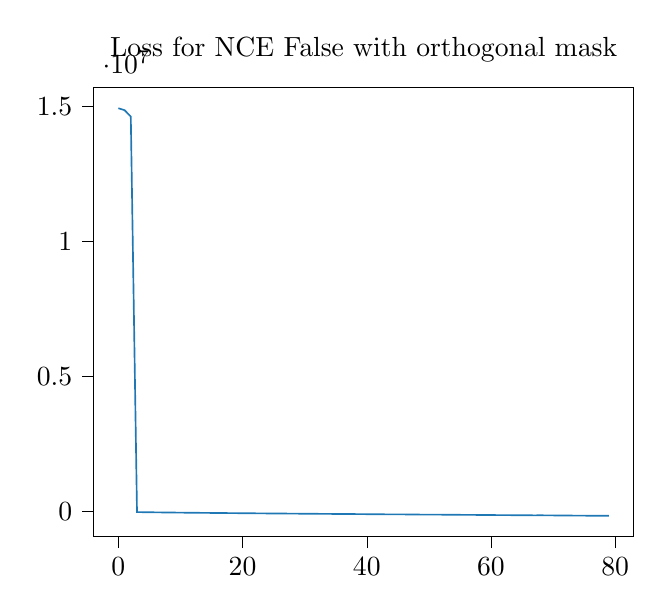
\begin{tikzpicture}

\definecolor{color0}{rgb}{0.12156862745098,0.466666666666667,0.705882352941177}

\begin{axis}[
tick align=outside,
tick pos=left,
title={Loss for NCE False with orthogonal mask},
x grid style={white!69.0196078431373!black},
xmin=-3.95, xmax=82.95,
xtick style={color=black},
y grid style={white!69.0196078431373!black},
ymin=-906312.213716807, ymax=15676596.7979696,
ytick style={color=black}
]
\addplot [semithick, color0]
table {%
0 14922828.2065293
1 14851322.0153235
2 14613628.1243846
3 -14924.0312438251
4 -18325.4300028998
5 -21526.0714124805
6 -24439.5292240158
7 -27215.2974540656
8 -29855.2113649352
9 -32400.6446478801
10 -34993.8804898312
11 -37333.903464459
12 -39746.8203947197
13 -41990.7105366933
14 -44087.6691429382
15 -46056.2093561942
16 -48171.1686182579
17 -50417.1724380575
18 -52264.1077266666
19 -54356.2635831562
20 -56468.47839116
21 -57976.144394764
22 -60414.5639933364
23 -62704.6239484305
24 -64425.4038137519
25 -66106.99281673
26 -68176.2359662242
27 -69720.824769196
28 -71281.3497486823
29 -73304.7512832187
30 -75357.1371885734
31 -77657.0046706549
32 -78713.9164210394
33 -81048.1241685911
34 -81963.8399462666
35 -83603.2805701209
36 -86133.3932952854
37 -87541.3213781795
38 -87975.2354536352
39 -90758.5584489338
40 -91946.4280692278
41 -94516.330204542
42 -95430.0163919909
43 -98004.1524679738
44 -99778.2208729671
45 -99757.6351703303
46 -100667.070211765
47 -102508.036159486
48 -105472.492962282
49 -108368.703798614
50 -108504.221207585
51 -109477.628041207
52 -109983.3324171
53 -113582.567708837
54 -115556.140089701
55 -116068.211990037
56 -117040.870646596
57 -118187.692409934
58 -120430.565149049
59 -122202.171431519
60 -124473.800338794
61 -125706.5250792
62 -125802.773463053
63 -128334.852060357
64 -130914.556999674
65 -132259.232989933
66 -132931.807576448
67 -135387.14694955
68 -133352.156514522
69 -136343.769820478
70 -137656.789977815
71 -141209.845412414
72 -143195.836710575
73 -143789.548614026
74 -144782.694850325
75 -146340.188417037
76 -149886.339763313
77 -149537.358239353
78 -152543.622276516
79 -149220.345394974
};
\end{axis}

\end{tikzpicture}

		\caption{4-connected}
	\end{subfigure}
	\hfill
	\begin{subfigure}[b]{0.49\textwidth}
		% This file was created by tikzplotlib v0.9.6.
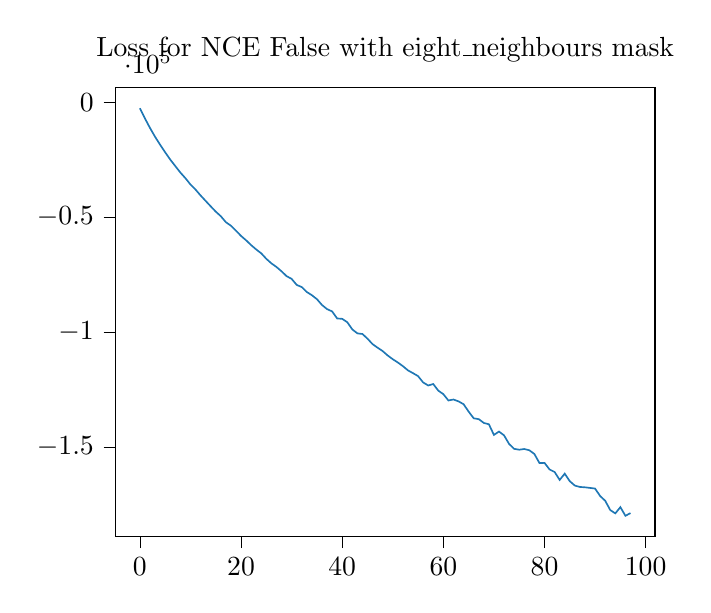
\begin{tikzpicture}

\definecolor{color0}{rgb}{0.12156862745098,0.466666666666667,0.705882352941177}

\begin{axis}[
tick align=outside,
tick pos=left,
title={Loss for NCE False with eight\_neighbours mask},
x grid style={white!69.0196078431373!black},
xmin=-4.85, xmax=101.85,
xtick style={color=black},
y grid style={white!69.0196078431373!black},
ymin=-188670.375161258, ymax=6192.23320793127,
ytick style={color=black}
]
\addplot [semithick, color0]
table {%
0 -2665.15808157732
1 -7112.69260307286
2 -11253.5285325134
3 -15075.8113468587
4 -18529.934408162
5 -21832.3660071646
6 -24975.0122924212
7 -27803.5312949652
8 -30615.3311349602
9 -33060.6332517976
10 -35811.0342236718
11 -38023.5599882992
12 -40573.5771738606
13 -42939.8143175122
14 -45299.9858275136
15 -47605.238840326
16 -49595.7566367541
17 -52191.7720793607
18 -53732.8193864293
19 -55879.2552938209
20 -58170.1826388766
21 -60062.5970431808
22 -62172.6742867518
23 -64052.3854118971
24 -65745.3761071861
25 -68120.6855907976
26 -70089.9880738746
27 -71650.2889727573
28 -73533.0311206946
29 -75637.8784369235
30 -76828.036290711
31 -79447.9902476299
32 -80389.5366598086
33 -82523.0667182633
34 -83928.9816961894
35 -85644.4640846767
36 -88166.2818431345
37 -89967.2238409397
38 -90952.9960620307
39 -94033.4012084403
40 -94204.8658787044
41 -95652.2551177471
42 -98798.7901959491
43 -100518.120729863
44 -100785.183778551
45 -102809.169264836
46 -105193.555814034
47 -106750.007411124
48 -108223.276004209
49 -110134.574929195
50 -111753.011671553
51 -113171.53794369
52 -114755.504364545
53 -116594.195388742
54 -117808.756717986
55 -119095.02393773
56 -121837.642380477
57 -123166.716630776
58 -122526.539828277
59 -125402.160171384
60 -126937.403484451
61 -129683.274187263
62 -129261.744053007
63 -130066.84615851
64 -131304.620290442
65 -134535.994864487
66 -137427.589870224
67 -137802.486743057
68 -139443.655985432
69 -140019.761486443
70 -144651.541449519
71 -143193.799724855
72 -144848.51897936
73 -148588.028358401
74 -150708.192654732
75 -151078.429973516
76 -150777.670656562
77 -151318.192658944
78 -152940.014231731
79 -156879.193147485
80 -156811.486141
81 -159667.595185268
82 -160772.173703344
83 -164213.602116366
84 -161480.632235731
85 -164774.094239158
86 -166680.866984232
87 -167275.392322074
88 -167422.602190752
89 -167691.575657162
90 -167965.071541737
91 -171222.303312684
92 -173270.261837716
93 -177325.470067554
94 -178751.055678833
95 -176046.449765888
96 -179812.983871749
97 -178624.772910044
};
\end{axis}

\end{tikzpicture}

		\caption{8-connected}
	\end{subfigure}
	\caption{Loss (SM)}
	\label{loss_SM_fig}
\end{figure}




\section*{\center Exercise 2}

The first step was to extract 50,000 image patches of resolution $28\times 28$. We solved this problem by running the following loop: In each iteration, an image from the \texttt{Flickr30k} dataset is loaded, converted to grayscale, and split into multiple patches using the method \texttt{tf.image.extract\_patches}. Two such patches are selected at random and saved, before moving on to the next iteration, and the program terminates after saving 50,000 patches. See \texttt{create\_image\_patches.py} for details.

Next, we computed a constrained Gaussian representing the above data \lipsum[2]































\end{document}